%% ============================================================
%% Relatório Técnico — Trabalho Final de Ciência de Dados (TP2)
%% Tema 1: Cobertura vacinal e mortalidade infantil por região
%%
%% Este arquivo foi escrito para ser colado como main.tex dentro
%% do projeto Overleaf criado a partir do "Springer Nature LaTeX
%% Template" (sn-jnl.cls, sn-mathphys-num.bst e demais arquivos
%% de suporte já devem estar no projeto). Copie a pasta "figuras"
%% para a raiz do projeto Overleaf.
%% ============================================================
\documentclass[pdflatex,sn-mathphys-num]{sn-jnl}
\usepackage{amsmath}
\usepackage{graphicx}
\usepackage{booktabs}
\usepackage{multirow}
\usepackage[T1]{fontenc}
\usepackage[utf8]{inputenc}
\usepackage[brazilian]{babel}
\raggedbottom

%% Tentativa opcional de traduzir o rótulo de "Keywords" para
%% "Palavras-chave". NÃO testado contra a versão exata do sn-jnl.cls
%% deste projeto — se a compilação quebrar com "Undefined control
%% sequence \keywordname", comente a linha abaixo e mantenha
%% "Keywords" em inglês (é comum em artigos em português que usam
%% templates internacionais, não é um erro grave).
% \renewcommand{\keywordname}{Palavras-chave}

\begin{document}

\title[Cobertura vacinal e mortalidade infantil]{Cobertura vacinal e mortalidade infantil por região}

\author*[1]{\fnm{Kauã} \sur{Guimarães Esperança Moreira}}\email{kaua.guimaraes@unesp.br}

\author[1]{\fnm{Samuel} \sur{Souza Del Grande}}\email{samuel.grande@unesp.br}

\affil*[1]{\orgdiv{Faculdade de Ciências}, \orgname{Universidade Estadual Paulista (UNESP)}, \orgaddress{\city{Bauru}, \state{SP}, \country{Brasil}}}

\abstract{A imunização infantil é um dos pilares da saúde pública, mas a cobertura vacinal varia consideravelmente entre os municípios brasileiros. Este trabalho investiga se essa variação está associada a diferenças na mortalidade infantil, e se a mortalidade em si varia de forma consistente entre as regiões do país. A partir de bases públicas do Ministério da Saúde/DATASUS (PNI, SINASC e SIM) referentes a 2022, foi construída uma base municipal unificada (n = 4.062 municípios) combinando cobertura vacinal contra poliomielite, nascidos vivos e óbitos infantis, a partir da qual se calculou uma taxa de mortalidade infantil por 1.000 nascidos vivos. A análise exploratória revelou grande dispersão na cobertura vacinal (média de 89,9\%, com 27,4\% dos municípios acima de 100\%, sinal de inconsistência de registro) e na mortalidade (mediana de 14,3 óbitos por 1.000 nascidos vivos). A correlação de Spearman entre cobertura vacinal e mortalidade foi positiva mas muito fraca ($\rho = 0{,}085$; $p < 0{,}001$) e deixou de ser estatisticamente significativa ($\rho = -0{,}022$; $p = 0{,}22$) em uma análise de sensibilidade restrita a municípios com pelo menos 100 nascidos vivos, evidenciando que o resultado inicial é dominado por instabilidade estatística em municípios pequenos. Por outro lado, o teste de Kruskal-Wallis identificou diferenças significativas na mortalidade entre regiões ($H = 25{,}29$; $p < 0{,}001$), concentradas principalmente entre a região Norte e o Sudeste e entre o Nordeste e o Sudeste. Concluímos que os dados de 2022 não sustentam uma relação direta e robusta entre cobertura vacinal contra poliomielite e mortalidade infantil no nível municipal, e que a atenção de política pública deveria se voltar às desigualdades regionais de mortalidade e à qualidade do próprio registro de cobertura vacinal, e não a uma leitura causal simplista entre as duas variáveis.}


\maketitle

\noindent\textbf{Palavras-chave:} cobertura vacinal, poliomielite, mortalidade infantil, DATASUS, ciência de dados, saúde pública

\noindent\small\emph{Repositório:} \url{https://github.com/deltageneral186/Projeto-Final-de-Ciencia-de-Dados}


\vspace{1em}

\section{Introdução}\label{sec:intro}

A vacinação infantil é reconhecida como uma das intervenções de saúde pública de melhor relação custo-benefício, e campanhas de imunização contra a poliomielite fazem parte da rotina do Programa Nacional de Imunizações (PNI) no Brasil desde a década de 1980. Apesar disso, a cobertura vacinal registrada nos municípios brasileiros é bastante heterogênea: municípios vizinhos, e até mesmo municípios de uma mesma microrregião, podem apresentar coberturas muito distintas, refletindo diferenças de infraestrutura de saúde, de mobilização das equipes de atenção básica e, também, de qualidade do próprio registro administrativo.

Este trabalho parte de uma pergunta relativamente direta, mas relevante do ponto de vista de gestão em saúde: \emph{existe relação entre a cobertura vacinal contra poliomielite e a taxa de mortalidade entre municípios e regiões brasileiras?} Se municípios com cobertura vacinal mais baixa também apresentassem sistematicamente mortalidade mais alta, isso reforçaria o argumento para priorizar recursos de vigilância epidemiológica e busca ativa de crianças não vacinadas nesses locais. Se, por outro lado, essa relação não se sustentar nos dados, isso sugere que fatores de mortalidade infantil e de cobertura vacinal, embora ambos relacionados à saúde materno-infantil, podem estar respondendo a determinantes distintos — o que também é uma informação relevante para o desenho de políticas.

Do ponto de vista epidemiológico, é razoável esperar alguma relação entre cobertura vacinal e mortalidade infantil: a poliomielite em si já foi eliminada como causa relevante de óbito no Brasil, mas municípios com baixa cobertura vacinal tendem, em tese, a ser também municípios com menor capilaridade da atenção básica, menor acesso a pré-natal, parto assistido e puericultura — fatores diretamente ligados à mortalidade infantil por outras causas. Sob essa hipótese, a cobertura vacinal funcionaria menos como causa direta da mortalidade e mais como um \emph{proxy} da qualidade geral da rede de atenção à saúde materno-infantil do município. É essa hipótese indireta que a análise a seguir busca testar empiricamente, e não uma relação causal direta entre a vacina contra poliomielite e a sobrevida infantil.

O restante deste relatório está organizado da seguinte forma: a Seção~\ref{sec:dados} descreve os dados utilizados e a metodologia de tratamento e análise; a Seção~\ref{sec:resultados} apresenta os resultados da análise exploratória e dos testes estatísticos; a Seção~\ref{sec:limitacoes} discute as limitações do estudo; e a Seção~\ref{sec:conclusao} traz a conclusão e a recomendação final.

\section{Dados e Metodologia}\label{sec:dados}

\subsection{Fontes de dados}

Foram utilizadas três bases públicas do Ministério da Saúde, disponibilizadas via DATASUS/TabNet (\url{https://datasus.saude.gov.br/informacoes-de-saude-tabnet/}), todas referentes ao ano de 2022 e agregadas por município:

\begin{itemize}
\item \textbf{Cobertura vacinal contra poliomielite} — Sistema do Programa Nacional de Imunizações (PNI), com o percentual de cobertura vacinal por município (arquivo \texttt{ImunizaçãoPorMunicípio2022.csv});
\item \textbf{Nascidos vivos} — Sistema de Informações sobre Nascidos Vivos (SINASC), com o número de nascidos vivos por município de residência da mãe (arquivo \texttt{NascidosVivosPorMunicípio2022.csv});
\item \textbf{Óbitos infantis} — Sistema de Informações sobre Mortalidade (SIM), com o número de óbitos de menores de 1 ano por município de residência (arquivo \texttt{ÓbitosPorMunicípio2022.csv});
\end{itemize}

Os três arquivos, o notebook Jupyter com o código completo e o \texttt{README.md} do projeto estão disponíveis no repositório público do trabalho.\footnote{\url{https://github.com/deltageneral186/Projeto-Final-de-Ciencia-de-Dados}} Os dados não contêm informação pessoal identificável: todos os indicadores são agregados por município, em conformidade com as diretrizes de dados e ética do trabalho.

\subsection{Tratamento e integração dos dados}

Os arquivos originais do TabNet trazem cabeçalhos e rodapés descritivos, totais gerais e uma linha de dados ignorados/incompletos, que não correspondem a municípios válidos. O tratamento aplicado consistiu em:

\begin{enumerate}
\item leitura dos arquivos com o separador \texttt{;} e codificação \texttt{latin1}, características do exportador do TabNet;
\item filtragem das linhas cujo campo de município segue o padrão \emph{código IBGE de 6 dígitos + nome} (expressão regular \texttt{\^{}\textbackslash d\{6\}\textbackslash s}), o que remove automaticamente linhas de total, cabeçalho e notas de rodapé;
\item conversão do percentual de cobertura vacinal de formato brasileiro (vírgula decimal) para ponto decimal e para tipo numérico;
\item extração do código IBGE de 6 dígitos de cada município, usado como chave de junção entre as três bases;
\item junção (\emph{inner join}) das três bases pelo código do município, restando apenas municípios presentes simultaneamente nas três fontes;
\item mapeamento do código do município para a Unidade da Federação (dois primeiros dígitos do código IBGE) e desta para a respectiva região (Norte, Nordeste, Centro-Oeste, Sudeste, Sul).
\end{enumerate}

A base final resultante contém $n = 4{.}062$ municípios com informação completa de cobertura vacinal, nascidos vivos e óbitos infantis, sem valores ausentes nas variáveis analisadas. A partir dela foi construída a variável de interesse — a taxa de mortalidade infantil municipal, definida como

\begin{equation}
\text{Taxa de Mortalidade Infantil} = \frac{\text{Óbitos infantis}}{\text{Nascidos Vivos}} \times 1{.}000 ,
\label{eq:taxa}
\end{equation}

isto é, óbitos de menores de 1 ano por 1.000 nascidos vivos no município no ano de 2022. A base do SIM utilizada já foi extraída com o filtro etário de menores de 1 ano, de modo que a taxa calculada corresponde à definição usual de taxa de mortalidade infantil, e não a um indicador de mortalidade geral.

\subsection{Técnicas de análise}

Além da análise exploratória de dados (EDA) — estatística descritiva geral e por região, identificação de valores atípicos e visualizações — foram aplicadas as seguintes técnicas formais, escolhidas por serem adequadas a variáveis com distribuição assimétrica e à comparação de mais de dois grupos independentes:

\begin{itemize}
\item \textbf{Correlação de Spearman} entre cobertura vacinal e taxa de mortalidade infantil, por ser uma medida não paramétrica de associação monotônica, robusta a distribuições assimétricas e a valores extremos;
\item \textbf{Teste de Kruskal-Wallis} para comparar a distribuição da taxa de mortalidade infantil entre as cinco regiões brasileiras, alternativa não paramétrica à ANOVA de um fator;
\item \textbf{Testes post-hoc de Mann-Whitney} par a par entre regiões, com correção de Holm-Bonferroni para comparações múltiplas, de modo a identificar especificamente quais pares de região diferem entre si após o resultado global do Kruskal-Wallis;
\item \textbf{Análise de sensibilidade}, repetindo a correlação de Spearman apenas para municípios com pelo menos 100 nascidos vivos em 2022, para avaliar o quanto o resultado inicial é influenciado por municípios pequenos, nos quais a taxa de mortalidade infantil é numericamente instável (poucos nascimentos fazem a taxa saltar de forma desproporcional a cada óbito adicional).
\end{itemize}

Em todos os testes de hipótese adotou-se o nível de significância convencional de $\alpha = 0{,}05$. Todo o processamento foi realizado em Python (\texttt{pandas}, \texttt{numpy}, \texttt{scipy}, \texttt{statsmodels}, \texttt{matplotlib} e \texttt{seaborn}), com código, ambiente de dependências (\texttt{requirements.txt}) e histórico de commits disponíveis no repositório Git do projeto.

\section{Resultados}\label{sec:resultados}

\subsection{Estatística descritiva geral}

A Tabela~\ref{tab:desc} resume as quatro variáveis centrais da base final. A cobertura vacinal contra poliomielite apresentou média de 89,9\% (desvio padrão de 22,0 pontos percentuais), com forte dispersão: o mínimo registrado foi de 12,1\% e o máximo de 316,0\%. Esse máximo muito acima de 100\% já é, por si, um indício de inconsistência no registro administrativo em alguns municípios, discutido na Seção~\ref{sec:limitacoes}. A taxa de mortalidade infantil apresentou média de 17,7 óbitos por 1.000 nascidos vivos e mediana de 14,3, com máximo de 166,7 — valor tipicamente associado a municípios muito pequenos, nos quais um único óbito já desloca fortemente a taxa.

\begin{table}[h]
\centering
\caption{Estatística descritiva das variáveis analisadas (n = 4.062 municípios, dados de 2022).}\label{tab:desc}
\begin{tabular}{@{}lrrrr@{}}
\toprule
Variável & Média & Mediana & Desvio padrão & Máximo \\
\midrule
Cobertura vacinal (\%) & 89,87 & 88,53 & 22,03 & 316,00 \\
Nascidos vivos & 607,12 & 204,00 & 2.805,75 & 132.050 \\
Óbitos infantis & 7,94 & 3,00 & 32,56 & 1.437 \\
Taxa de mortalidade infantil (por 1.000) & 17,71 & 14,29 & 12,78 & 166,67 \\
\botrule
\end{tabular}
\end{table}

Dois pontos chamaram atenção na EDA e motivaram uma investigação específica de valores atípicos: (i) 1.114 municípios (27,4\% da base) registraram cobertura vacinal acima de 100\%, distribuídos de forma desigual entre as regiões, com maior concentração relativa no Nordeste (444 municípios) e no Sudeste (306); e (ii) 361 municípios (8,9\%) tiveram menos de 50 nascidos vivos em 2022, e 1.004 (24,7\%) tiveram menos de 100 — nesses casos, a taxa de mortalidade infantil por 1.000 nascidos vivos tende a ser numericamente instável, pois cada óbito adicional desloca a taxa em uma magnitude muito maior do que em municípios grandes.

\subsection{Investigação de valores atípicos}\label{sec:outliers}

Para entender a origem desses dois padrões, examinamos diretamente os municípios nos extremos das distribuições. A Tabela~\ref{tab:top_cobertura} lista os dez municípios com maior cobertura vacinal registrada em 2022: todos apresentam cobertura acima de 175\% e, sem exceção, todos têm um número muito pequeno de nascidos vivos no ano (entre 22 e 126). Isso é consistente com a hipótese de que a cobertura acima de 100\% pode estar relacionada a diferenças entre a população-alvo estimada utilizada no cálculo da cobertura e a população efetivamente registrada no município — o que reforça a necessidade de cautela ao interpretar a cobertura vacinal como indicador comparável entre municípios de porte muito diferente.

\begin{table}[h]
\centering
\caption{Os dez municípios com maior cobertura vacinal contra poliomielite registrada em 2022.}\label{tab:top_cobertura}
\begin{tabular}{@{}llrr@{}}
\toprule
Município & Região & Cobertura (\%) & Nascidos vivos \\
\midrule
Sucupira do Riachão & Nordeste & 316,00 & 30 \\
Leandro Ferreira & Sudeste & 235,00 & 29 \\
Ichu & Nordeste & 230,77 & 56 \\
Nova Aurora & Centro-Oeste & 228,57 & 22 \\
Santa Cecília do Sul & Sul & 220,00 & 28 \\
Talismã & Norte & 208,70 & 28 \\
São Domingos do Azeitão & Nordeste & 200,00 & 126 \\
Joca Claudino & Nordeste & 192,86 & 30 \\
Nova Marilândia & Centro-Oeste & 181,82 & 50 \\
Pratinha & Sudeste & 175,76 & 31 \\
\botrule
\end{tabular}
\end{table}

O mesmo padrão aparece na ponta oposta: os dez municípios com maior taxa de mortalidade infantil em 2022 têm, todos, menos de 42 nascidos vivos e, em geral, apenas 1 ou 2 óbitos — por exemplo, Vanini (RS), com 2 óbitos em 12 nascidos vivos, atinge uma taxa de 166,7 por 1.000, o maior valor da base. Em contraste, quando olhamos apenas para municípios de porte médio a grande (pelo menos 100 nascidos vivos), as menores taxas de mortalidade infantil da base — como Breu Branco (PA) e Morrinhos (GO), ambos com um único óbito em mais de 600 nascidos vivos — também aparecem, mas de forma numericamente muito mais estável e interpretável. Esse contraste ilustra concretamente por que a análise de sensibilidade da Seção~\ref{sec:resultados} restringe a amostra a municípios com pelo menos 100 nascidos vivos: nos municípios menores, tanto a cobertura vacinal quanto a taxa de mortalidade infantil são dominadas por ruído estatístico decorrente do pequeno tamanho da população de base, e não necessariamente por diferenças reais na qualidade da atenção à saúde.

\subsection{Diferenças regionais}

A Tabela~\ref{tab:regiao} apresenta o resumo de cobertura vacinal e mortalidade infantil por região. A região Norte apresentou a menor cobertura vacinal média (80,3\%) entre as cinco regiões, enquanto Centro-Oeste, Nordeste e Sul ficaram próximas de 91--92\%. Em relação à mortalidade infantil, a região Norte também apresentou a maior mediana (15,8 óbitos por 1.000 nascidos vivos), seguida pelo Nordeste (14,8), enquanto o Sudeste apresentou a menor mediana (13,3).

\begin{table}[h]
\centering
\caption{Cobertura vacinal e taxa de mortalidade infantil por região (médias e medianas).}\label{tab:regiao}
\footnotesize
\begin{tabular}{@{}lrrrrr@{}}
\toprule
Região & Municípios & Cobertura (\%) média & Cobertura (\%) mediana & Mort. infantil média & Mort. infantil mediana \\
\midrule
Centro-Oeste & 334 & 92,85 & 89,83 & 19,52 & 14,29 \\
Nordeste & 1.476 & 91,32 & 90,58 & 17,43 & 14,80 \\
Norte & 376 & 80,27 & 80,22 & 18,01 & 15,82 \\
Sudeste & 1.146 & 89,33 & 87,69 & 17,00 & 13,33 \\
Sul & 730 & 91,37 & 89,07 & 18,44 & 13,93 \\
\botrule
\end{tabular}
\end{table}

As Figuras~\ref{fig:cobertura_regiao} e~\ref{fig:mortalidade_regiao} ilustram essa dispersão por meio de boxplots. A cobertura vacinal na região Norte não apenas tem a menor mediana como também a menor dispersão relativa acima de 100\%, enquanto Nordeste e Sudeste concentram mais casos de cobertura aparentemente superestimada. Já a distribuição da mortalidade infantil (Figura~\ref{fig:mortalidade_regiao}) mostra caudas longas em todas as regiões, compatíveis com a presença de municípios pequenos com taxas extremas.

\begin{figure}[h]
\centering
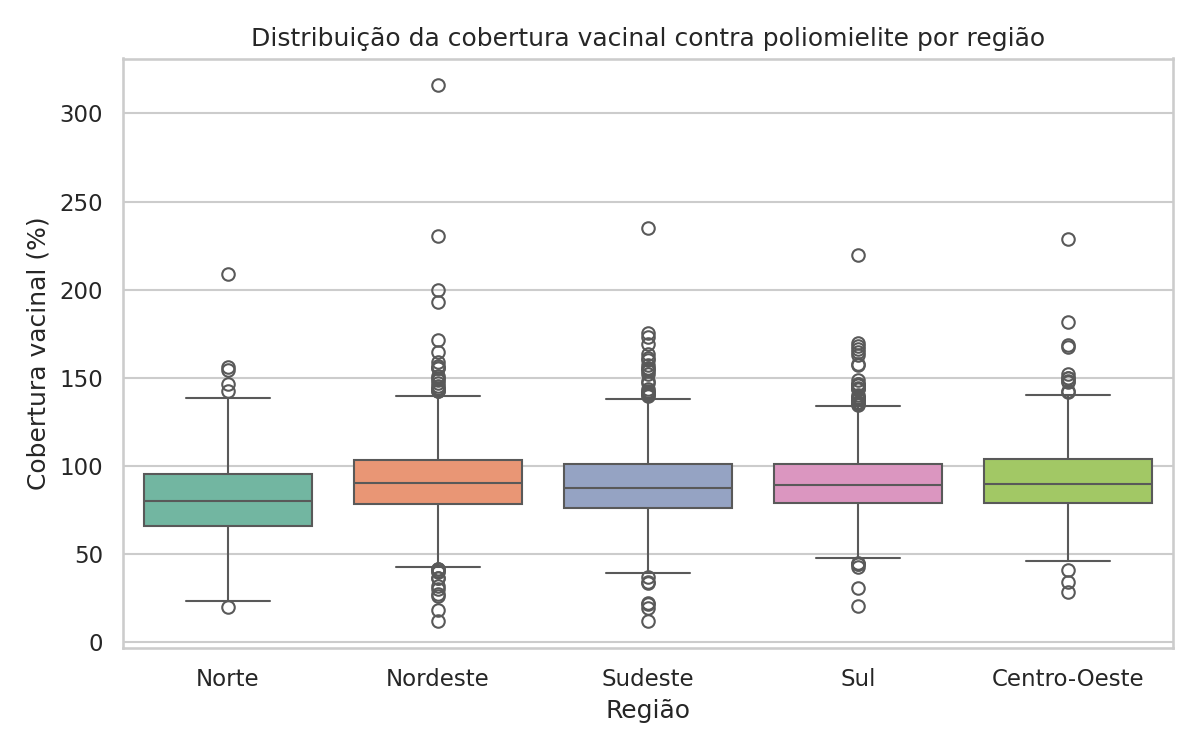
\includegraphics[width=0.85\textwidth]{figuras/fig_cobertura_regiao.png}
\caption{Distribuição da cobertura vacinal contra poliomielite por região (2022).}
\label{fig:cobertura_regiao}
\end{figure}

\begin{figure}[h]
\centering
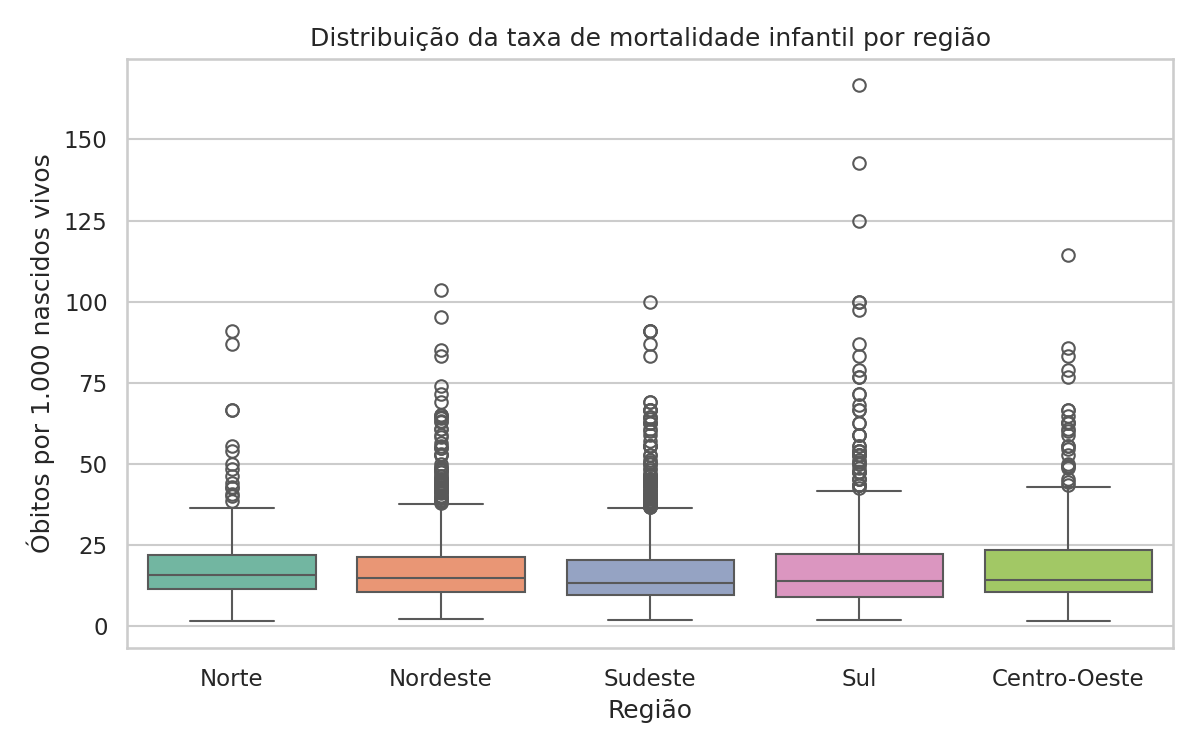
\includegraphics[width=0.85\textwidth]{figuras/fig_mortalidade_regiao.png}
\caption{Distribuição da taxa de mortalidade infantil por região (óbitos por 1.000 nascidos vivos, 2022).}
\label{fig:mortalidade_regiao}
\end{figure}

A Figura~\ref{fig:hist_mortalidade} mostra a distribuição geral da taxa de mortalidade infantil entre os 4.062 municípios: uma distribuição assimétrica à direita, com a maior parte dos municípios concentrada entre 5 e 25 óbitos por 1.000 nascidos vivos, e uma cauda de municípios com taxas muito mais altas — justamente os municípios menores. Essa assimetria é a razão pela qual optamos por técnicas não paramétricas (Spearman, Kruskal-Wallis, Mann-Whitney) em vez de testes que assumem normalidade.

\begin{figure}[h]
\centering
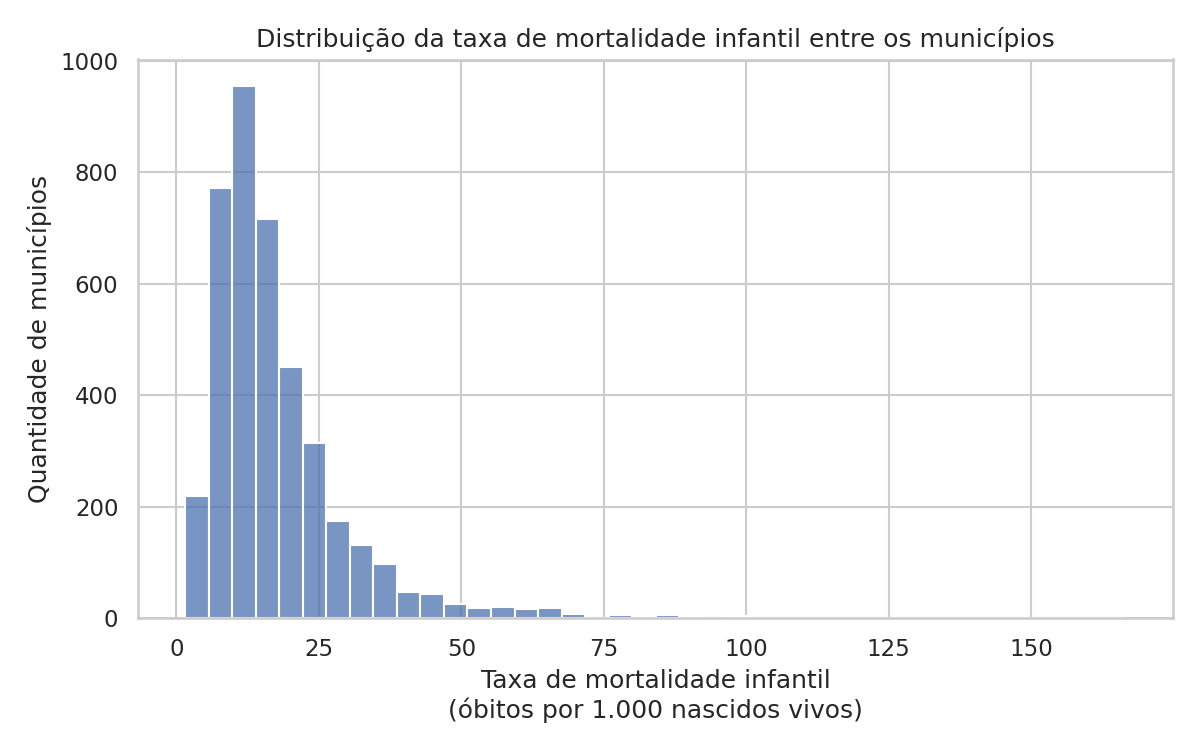
\includegraphics[width=0.85\textwidth]{figuras/fig_hist_mortalidade.png}
\caption{Distribuição da taxa de mortalidade infantil entre os municípios (2022).}
\label{fig:hist_mortalidade}
\end{figure}

\subsection{Cobertura vacinal x mortalidade infantil}

A Figura~\ref{fig:dispersao} apresenta a relação entre cobertura vacinal e taxa de mortalidade infantil em nível municipal, colorida por região. Visualmente, não há um padrão claro de queda da mortalidade à medida que a cobertura vacinal aumenta — a nuvem de pontos é praticamente horizontal, com grande dispersão vertical em toda a faixa de cobertura.

\begin{figure}[h]
\centering
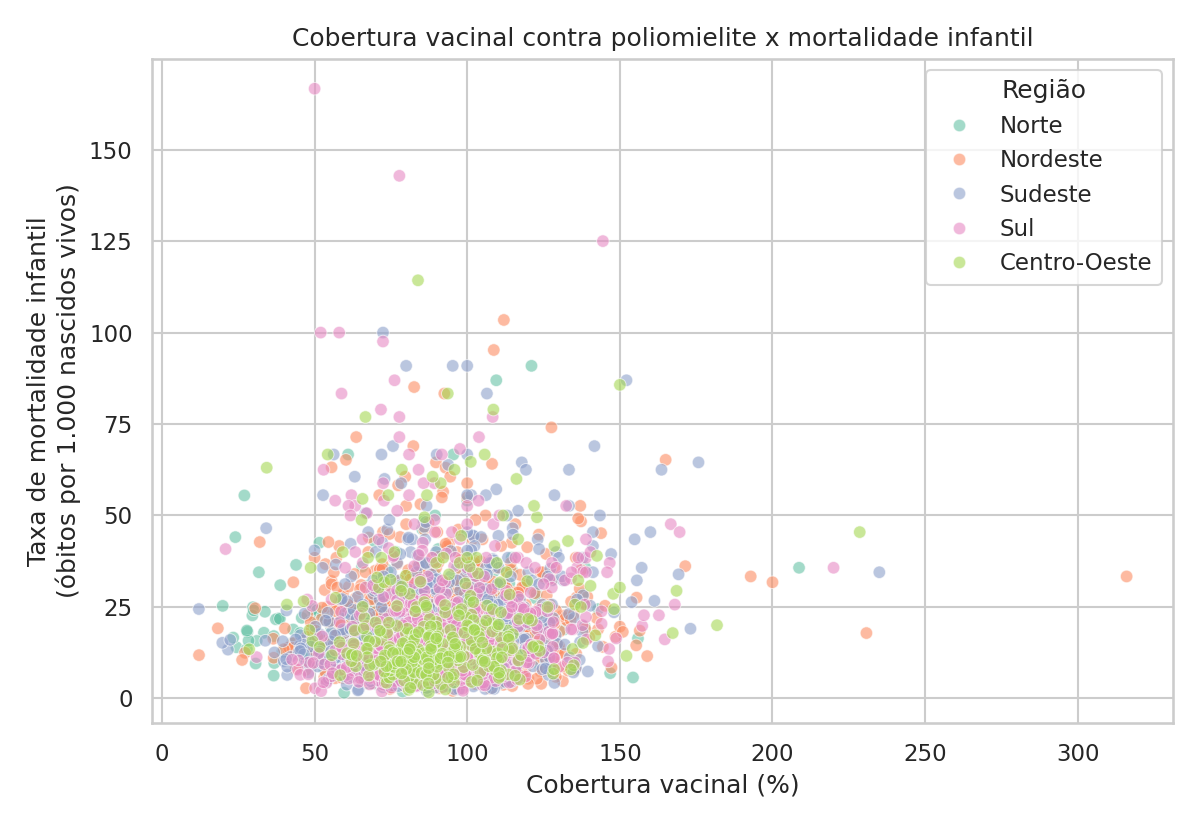
\includegraphics[width=0.85\textwidth]{figuras/fig_dispersao.png}
\caption{Cobertura vacinal contra poliomielite e taxa de mortalidade infantil, por município (2022).}
\label{fig:dispersao}
\end{figure}

Essa impressão visual foi confirmada pelo teste de correlação de Spearman entre cobertura vacinal e taxa de mortalidade infantil, considerando toda a base ($n = 4{.}062$): $\rho = 0{,}085$ ($p = 6{,}3 \times 10^{-8}$). A correlação é estatisticamente significativa — o que era esperado dado o tamanho da amostra — mas sua magnitude é considerada, na prática, desprezível: valores de $|\rho|$ abaixo de 0,1 indicam ausência de associação relevante entre as variáveis, mesmo quando o teste rejeita a hipótese nula de correlação zero.

\subsection{Diferenças de mortalidade infantil entre regiões}

O teste de Kruskal-Wallis, aplicado à taxa de mortalidade infantil entre as cinco regiões, indicou diferença estatisticamente significativa na distribuição da variável entre pelo menos um par de regiões ($H = 25{,}29$; $g.l. = 4$; $p = 4{,}4 \times 10^{-5}$). A Tabela~\ref{tab:posthoc} apresenta os pares comparados na análise post-hoc; entre as dez comparações realizadas, três apresentaram significância após a correção de Holm (Tabela~\ref{tab:posthoc}): Norte x Sudeste, Nordeste x Sudeste e Norte x Sul. Os demais pares de região não apresentaram diferença estatisticamente significativa após a correção.

\begin{table}[h]
\centering
\caption{Comparações post-hoc de Mann-Whitney entre regiões (taxa de mortalidade infantil), com correção de Holm-Bonferroni. Pares selecionados da comparação post-hoc; os três primeiros apresentam diferença estatisticamente significativa ($p_{\text{ajustado}} < 0{,}05$).}\label{tab:posthoc}
\begin{tabular}{@{}llrl@{}}
\toprule
Região 1 & Região 2 & $p$ ajustado (Holm) & Significativo \\
\midrule
Norte & Sudeste & 0,00047 & Sim \\
Nordeste & Sudeste & 0,00136 & Sim \\
Norte & Sul & 0,03936 & Sim \\
Sudeste & Centro-Oeste & 0,06258 & Não \\
Nordeste & Sul & 0,15987 & Não \\
\botrule
\end{tabular}
\end{table}

Em conjunto, esses resultados sugerem que as diferenças de mortalidade infantil entre regiões são reais e estatisticamente detectáveis — sobretudo a diferença entre o Sudeste (menor mortalidade) e o Norte e o Nordeste (maior mortalidade) —, mas que essas diferenças regionais não parecem ser explicadas pela cobertura vacinal contra poliomielite, dada a correlação praticamente nula encontrada na subseção anterior. É importante notar que a região Norte, apesar de ter a menor cobertura vacinal média (Tabela~\ref{tab:regiao}), não é estatisticamente diferente do Nordeste em termos de mortalidade, e a Nordeste, por sua vez, tem cobertura vacinal média semelhante à do Sul e do Centro-Oeste — ou seja, o ranking de cobertura vacinal entre regiões não acompanha de forma consistente o ranking de mortalidade, o que é mais um indício, agora em nível regional, contra uma relação direta entre as duas variáveis.

\subsection{Análise de sensibilidade}

Para verificar se a correlação de Spearman encontrada na base completa era, na verdade, um artefato dos municípios com poucos nascimentos (nos quais a taxa de mortalidade infantil é instável), repetimos o teste considerando apenas os 3.058 municípios com pelo menos 100 nascidos vivos em 2022. Nessa sub-base, a correlação deixou de ser positiva e deixou de ser estatisticamente significativa: $\rho = -0{,}022$ ($p = 0{,}22$). Esse resultado é o achado mais importante do trabalho: a fraquíssima correlação positiva observada na base completa não se sustenta quando se remove o ruído estatístico dos municípios pequenos, o que reforça a conclusão de que não há evidência robusta de associação entre cobertura vacinal contra poliomielite e mortalidade infantil nos dados municipais de 2022.

\subsection{Síntese dos resultados}

A Tabela~\ref{tab:sintese} resume os quatro testes estatísticos aplicados neste trabalho, suas hipóteses e conclusões. A leitura conjunta dos quatro resultados é o que sustenta a conclusão do trabalho: isoladamente, o teste de Spearman na base completa poderia sugerir uma associação (ainda que fraca) entre cobertura vacinal e mortalidade infantil; mas a análise de sensibilidade mostra que essa associação não resiste à remoção do ruído estatístico dos municípios pequenos, enquanto o Kruskal-Wallis e o post-hoc mostram que a variação geográfica de mortalidade infantil é real, porém não acompanha o padrão geográfico da cobertura vacinal.

\begin{table}[h]
\centering
\caption{Síntese dos testes estatísticos aplicados.}\label{tab:sintese}
\begin{tabular}{@{}p{3.1cm}p{4.6cm}p{2.3cm}p{3cm}@{}}
\toprule
Teste & O que avalia & Resultado & Conclusão \\
\midrule
Spearman (base completa) & Associação entre cobertura vacinal e mortalidade infantil, $n=4.062$ & $\rho=0{,}085$; $p<0{,}001$ & Associação estatisticamente significativa, porém desprezível \\
Spearman (sensibilidade, $n \geq 100$ nasc.) & O mesmo, restrito a municípios maiores, $n=3.058$ & $\rho=-0{,}022$; $p=0{,}22$ & Associação deixa de ser significativa \\
Kruskal-Wallis & Diferença de mortalidade infantil entre 5 regiões & $H=25{,}29$; $p<0{,}001$ & Há diferença significativa entre regiões \\
Mann-Whitney + Holm (post-hoc) & Quais pares de região diferem entre si & 3 de 10 pares significativos & Diferença concentrada em Norte/Nordeste vs.\ Sudeste \\
\botrule
\end{tabular}
\end{table}

\section{Limitações}\label{sec:limitacoes}

Algumas limitações devem ser consideradas na interpretação dos resultados:

\begin{enumerate}
\item \textbf{Instabilidade em municípios pequenos.} Como discutido, quase um quarto dos municípios (24,7\%) teve menos de 100 nascidos vivos em 2022, o que torna a taxa de mortalidade infantil extremamente sensível a poucos óbitos. A análise de sensibilidade buscou mitigar esse problema, mas não o elimina por completo, já que mesmo o corte de 100 nascidos vivos ainda inclui municípios de porte pequeno.
\item \textbf{Qualidade do registro de cobertura vacinal.} A presença de 27,4\% dos municípios com cobertura vacinal acima de 100\% é um forte indício de problemas na estimativa do denominador populacional utilizado pelo PNI (população-alvo estimada) em nível municipal, um problema documentado na literatura de avaliação de coberturas vacinais no Brasil. Isso significa que parte da variável explicativa central do trabalho apresenta incerteza de mensuração, o que reduz a confiança na interpretação da associação encontrada.
\item \textbf{Desenho observacional e ausência de controle por confundidores.} Este trabalho é uma análise observacional e transversal (um único ano, 2022). Fatores socioeconômicos, de saneamento básico e de acesso a serviços de saúde — não incluídos nesta análise — provavelmente afetam tanto a cobertura vacinal quanto a mortalidade infantil, e podem mascarar ou distorcer a associação direta entre as duas variáveis. Os resultados aqui apresentados são, portanto, associativos, e não permitem qualquer inferência causal.
\item \textbf{Recorte temporal único.} A análise não avalia tendência ao longo do tempo; um único ano pode não ser representativo de padrões estruturais de mais longo prazo, especialmente em um contexto pós-pandêmico em que campanhas de vacinação sofreram interrupções significativas em 2020--2021.
\end{enumerate}

\section{Conclusão}\label{sec:conclusao}

Os dados municipais de 2022 não fornecem evidência robusta de uma relação direta entre a cobertura vacinal contra poliomielite e a taxa de mortalidade infantil no Brasil. A correlação de Spearman na base completa foi positiva mas de magnitude desprezível ($\rho = 0{,}085$) e, mais importante, deixou de ser estatisticamente significativa quando a análise foi restrita a municípios com pelo menos 100 nascidos vivos ($\rho = -0{,}022$; $p = 0{,}22$), indicando que o resultado inicial é sensível à inclusão de municípios pequenos e não se mantém na análise de sensibilidade. Por outro lado, há diferenças regionais de mortalidade infantil estatisticamente significativas — sobretudo entre o Sudeste (menor mortalidade) e as regiões Norte e Nordeste (maior mortalidade) —, que não podem ser atribuídas à cobertura vacinal contra poliomielite propriamente dita.

\textbf{Recomendação.} Com base nesses resultados, a recomendação técnica deste trabalho é que gestores de saúde não tratem a cobertura vacinal contra poliomielite, isoladamente, como um preditor confiável de mortalidade infantil em nível municipal para fins de priorização orçamentária. Em termos mais concretos, recomenda-se:

\begin{enumerate}
\item \textbf{Priorizar a investigação das disparidades regionais de mortalidade infantil}, e não da cobertura vacinal isoladamente, começando pelos pares de região com diferença estatisticamente confirmada neste trabalho (Norte e Nordeste versus Sudeste). Essa investigação deve incorporar variáveis não avaliadas aqui — acesso a pré-natal, saneamento básico, renda familiar e distância até unidades de saúde de referência — para identificar os determinantes reais por trás da diferença observada.
\item \textbf{Revisar a estimativa populacional de base usada no cálculo da cobertura vacinal} antes de utilizá-la para alocação de recursos ou avaliação de desempenho municipal, dado que mais de um quarto dos municípios (27,4\%) registrou cobertura acima de 100\% em 2022 — um problema de mensuração, não de excesso real de vacinação, e concentrado justamente nos municípios menores, como mostrado na Seção~\ref{sec:outliers}.
\item \textbf{Tratar indicadores municipais de mortalidade infantil com o devido cuidado estatístico em municípios pequenos}, evitando comparações diretas de taxas por 1.000 nascidos vivos entre municípios de porte muito distinto sem alguma forma de suavização, agregação regional ou intervalo de incerteza, já que a instabilidade dessas taxas em pequena escala foi um fator determinante para o enfraquecimento da correlação observada na análise de sensibilidade.
\end{enumerate}

Essas ressalvas sobre a qualidade e a granularidade do dado são, em si, um achado relevante de gestão, ainda que não respondam diretamente, em termos causais, à pergunta central do trabalho.

\section*{Declarações}

\textbf{Financiamento.} Não aplicável.

\noindent\textbf{Conflito de interesses.} Os autores declaram não haver conflito de interesses.

\noindent\textbf{Disponibilidade dos dados} Os dados utilizados (Cobertura vacinal, Nascidos vivos e Óbitos infantis por município, 2022) são públicos e estão disponíveis no TabNet/DATASUS (\url{https://datasus.saude.gov.br/informacoes-de-saude-tabnet/}) e também no repositório do projeto.

\noindent\textbf{Disponibilidade do código.} O código-fonte completo (notebook Jupyter), os dados utilizados e o arquivo de dependências estão disponíveis publicamente em \url{https://github.com/deltageneral186/Projeto-Final-de-Ciencia-de-Dados}.

\noindent\textbf{Contribuição dos autores.} Ambos os autores contribuíram igualmente para a concepção do trabalho, o tratamento e a análise dos dados, e a redação do relatório.

%% ============================================================
%% Referências — sn-mathphys-num.bst usa \begin{thebibliography}
%% Ajuste/expanda conforme a norma pedida pela disciplina.
%% ============================================================
\begin{thebibliography}{99}

\bibitem{datasus_pni} Ministério da Saúde/DATASUS. \emph{Sistema de Informações do Programa Nacional de Imunizações (PNI) — Cobertura Vacinal por Município, 2022}. Disponível em: \url{https://datasus.saude.gov.br/informacoes-de-saude-tabnet/}. Acesso em: 16 set. 2026.

\bibitem{datasus_sinasc} Ministério da Saúde/DATASUS. \emph{Sistema de Informações sobre Nascidos Vivos (SINASC) — Nascidos Vivos por Município, 2022}. Disponível em: \url{https://datasus.saude.gov.br/informacoes-de-saude-tabnet/}. Acesso em: 16 set. 2026.

\bibitem{datasus_sim} Ministério da Saúde/DATASUS. \emph{Sistema de Informações sobre Mortalidade (SIM) — Óbitos infantis por Município, 2022}. Disponível em: \url{https://datasus.saude.gov.br/informacoes-de-saude-tabnet/}. Acesso em: 16 set. 2026.

\bibitem{spearman1904} Spearman, C.: The proof and measurement of association between two things. Am. J. Psychol. \textbf{15}(1), 72--101 (1904).

\bibitem{kruskal1952} Kruskal, W.H., Wallis, W.A.: Use of ranks in one-criterion variance analysis. J. Am. Stat. Assoc. \textbf{47}(260), 583--621 (1952).

\bibitem{mannwhitney1947} Mann, H.B., Whitney, D.R.: On a test of whether one of two random variables is stochastically larger than the other. Ann. Math. Stat. \textbf{18}(1), 50--60 (1947).

\bibitem{holm1979} Holm, S.: A simple sequentially rejective multiple test procedure. Scand. J. Stat. \textbf{6}(2), 65--70 (1979).

\end{thebibliography}

\end{document}